\chapter{Arc Length of the Quadratic Curve as a Periodic Sequence}
\label{sec:bogenlaenge_parabel}

In the preceding chapters the arc length of the Archimedean spiral was
investigated. Here we return to the original quadratic curve
\[
  k(n) = \frac{2n^2 + 3n + 1}{6}
\]
and systematically compute its arc length along the integer
indices (i.e.\ $n \equiv 1, 5 \pmod{6}$, cf.\ Chapter~\ref{sec:arithmetik}).
The result is a closed-form formula that reproduces the same periodic
structure of twin and gap zones that already appeared in
Chapter~\ref{sec:arithmetik} as a difference sequence ---
now, however, as an \emph{arc-length sequence} of the parabola.

% ─────────────────────────────────────────────────────────────────────────────
\section{Derivation of the General Arc-Length Formula}
\label{sec:bl_herleitung}
% ─────────────────────────────────────────────────────────────────────────────

\subsection{Arc-Length Element of the Parabola}

For a real-valued function $k(n)$ the arc-length element is
\[
  ds = \sqrt{1 + \bigl[k'(n)\bigr]^2}\,dn.
\]
The derivative of the quadratic sequence is:
\[
  k'(n) = \frac{4n+3}{6}.
\]
This yields:
\[
  ds = \sqrt{1 + \frac{(4n+3)^2}{36}}\,dn
     = \frac{1}{6}\sqrt{36 + (4n+3)^2}\,dn.
\]

The arc length between two indices $n_1$ and $n_2$ is therefore:
\begin{equation}\label{eq:bl_parabel_integral}
  L(n_1, n_2)
  = \frac{1}{6}\int_{n_1}^{n_2} \sqrt{36 + (4n+3)^2}\,dn.
\end{equation}

\subsection{Substitution and Closed Form}

The integral~\eqref{eq:bl_parabel_integral} is reduced to a standard
integral by the linear substitution
\[
  u = 4n + 3, \qquad du = 4\,dn
\]
yielding:
\[
  L = \frac{1}{6} \cdot \frac{1}{4}
      \int_{u_1}^{u_2} \sqrt{u^2 + 36}\,du
  = \frac{1}{24}\int_{u_1}^{u_2} \sqrt{u^2 + 36}\,du,
\]
where $u_i = 4n_i + 3$.

The indefinite integral of $\sqrt{u^2 + a^2}$ is well known:
\[
  \int \sqrt{u^2 + a^2}\,du
  = \frac{1}{2}\Bigl[u\sqrt{u^2 + a^2}
    + a^2\ln\!\bigl(u + \sqrt{u^2+a^2}\bigr)\Bigr] + C.
\]
With $a = 6$ and the identity
$\ln(u + \sqrt{u^2+36}) = \operatorname{arcsinh}(u/6) + \ln 6$ (the constant
cancels upon evaluation), we obtain the antiderivative:
\[
  G(u) = \frac{1}{2}\Bigl[u\sqrt{u^2+36}
         + 36\operatorname{arcsinh}\!\left(\frac{u}{6}\right)\Bigr].
\]

\begin{theorem}[Closed-form arc-length formula for the parabola]\label{satz:bl_geschlossen}
Let $u_i = 4n_i + 3$. The arc length of the curve $k(n)$ between $n_1$
and $n_2$ is:
\begin{equation}\label{eq:bl_geschlossen}
  L(n_1, n_2)
  = \frac{1}{48}\Bigl[u\sqrt{u^2+36}
    + 36\operatorname{arcsinh}\!\left(\frac{u}{6}\right)
    \Bigr]_{u_1}^{u_2}.
\end{equation}
\end{theorem}

\begin{remark}[Alternative notation with $\operatorname{csch}^{-1}$]
Since $\operatorname{arcsinh}(x) = \operatorname{csch}^{-1}(1/x)$, the
formula can also be written as
\[
  L = \frac{1}{48}\Bigl[u\sqrt{u^2+36}
    + 36\operatorname{csch}^{-1}\!\!\left(\frac{6}{u}\right)
    \Bigr]_{u_1}^{u_2}.
\]
This form arises naturally from hyperbolic substitutions and is
the preferred output in some computer algebra systems.
\end{remark}

% ─────────────────────────────────────────────────────────────────────────────
\section{Twin-Zone Sequence (Minor Steps, \texorpdfstring{$\Delta n = 2$}{Δn = 2})}
\label{sec:twin_zone_bl}
% ─────────────────────────────────────────────────────────────────────────────

\subsection{Derivation of the Periodic Formula}

The minor steps connect $n_1 = 6m-1$ (with $n_1 \equiv 5 \pmod{6}$)
and $n_2 = 6m+1$ (with $n_2 \equiv 1 \pmod{6}$), for $m = 1, 2, 3, \ldots$
The corresponding $u$-values are:
\[
  u_1 = 4(6m-1)+3 = 24m - 1,
  \qquad
  u_2 = 4(6m+1)+3 = 24m + 7.
\]

\begin{theorem}[Twin-zone arc length]\label{satz:twin_zone}
The arc length of the parabola $k(n)$ over the $m$-th minor step
($n: 6m-1 \to 6m+1$) is:
\begin{multline}
  L_{\mathrm{Twin}}(m)
  = \frac{1}{48}\Bigl[
      (24m+7)\sqrt{(24m+7)^2+36}
    + 36\operatorname{arcsinh}\!\!\left(\frac{24m+7}{6}\right)
    \\
    - (24m-1)\sqrt{(24m-1)^2+36}
    - 36\operatorname{arcsinh}\!\!\left(\frac{24m-1}{6}\right)
    \Bigr].
\end{multline}
\end{theorem}

\begin{proof}
Direct application of Theorem~\ref{satz:bogenlaenge_geschlossen} with the bounds
$u_1 = 24m-1$ and $u_2 = 24m+7$.
\end{proof}

\subsection{Numerical Values}

\begin{table}[H]
\centering
\caption{Twin-zone arc lengths $L_{\mathrm{Twin}}(m)$ for the first
  seven periods. The arc length grows approximately linearly with $m$,
  with the ratio $L_{\mathrm{Twin}}(m) / \Delta_{\mathrm{Minor}}(m)$
  converging monotonically to~$1$.}
\renewcommand{\arraystretch}{1.2}
\begin{tabular}{cccccccc}
\toprule
$m$ & $n_1 \to n_2$ & $u_1$ & $u_2$ &
$\Delta_{\mathrm{Minor}}(m)$ & $L_{\mathrm{Twin}}(m)$ &
$L / \Delta_{\mathrm{Minor}}$ \\
\midrule
1 &  $5 \to  7$ & 23 &  31 &  9 &  9.2210749306 & 1.024564 \\
2 & $11 \to 13$ & 47 &  55 & 17 & 17.1174799293 & 1.006911 \\
3 & $17 \to 19$ & 71 &  79 & 25 & 25.0799476641 & 1.003198 \\
4 & $23 \to 25$ & 95 & 103 & 33 & 33.0605833402 & 1.001836 \\
5 & $29 \to 31$ & 119 & 127 & 41 & 41.0487686495 & 1.001189 \\
6 & $35 \to 37$ & 143 & 151 & 49 & 49.0408093942 & 1.000833 \\
7 & $41 \to 43$ & 167 & 175 & 57 & 57.0350833164 & 1.000615 \\
\bottomrule
\end{tabular}
\end{table}

\begin{remark}[Convergence to the minor step]
The last column shows that $L_{\mathrm{Twin}}(m) \to \Delta_{\mathrm{Minor}}(m)$
as $m \to \infty$. This is geometrically plausible: for large $m$ the
curve $k(n)$ in the short interval $[6m-1, 6m+1]$ is nearly rectilinear
(the curvature decreases), so the arc length converges to the chord length.
Since for very steep curves ($k'(n) \gg 1$) the arc length is asymptotically
dominated by the $k'$-term:
\[
  L_{\mathrm{Twin}}(m) \approx \int_{6m-1}^{6m+1} \frac{4n+3}{6}\,dn
  = \frac{1}{6}\Bigl[\frac{(4n+3)^2}{8}\Bigr]_{6m-1}^{6m+1}
  \approx 8m+1 = \Delta_{\mathrm{Minor}}(m).
\]
\end{remark}

\begin{figure}[H]
  \centering
  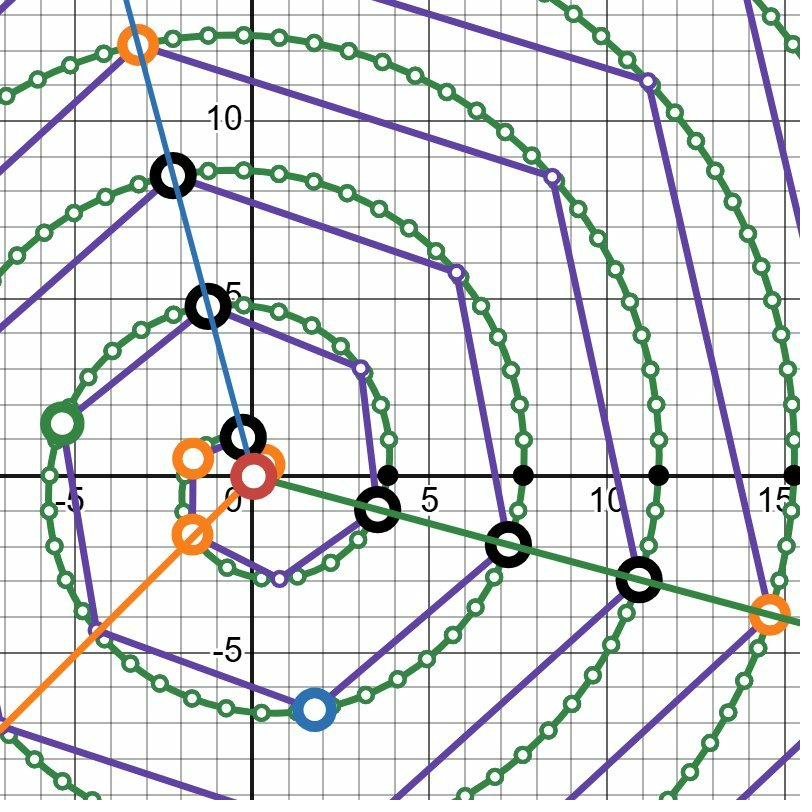
\includegraphics[width=0.88\textwidth]{bilder/spirale_zoom_bogenlaenge}
  \caption{Enlarged plan view of the Archimedean spiral
    $r = \tfrac{6}{\pi^2}\,\theta$ with equidistant arc-length scaling
    ($1\text{ unit} = 1$). The small green circular markers are placed at constant arc
    spacing~$1$ and are thus directly countable. The large hollow black dots mark
    the integer sequence values $k(n)$ on the spiral; the coloured
    hollow dots identify the same values on their respective diagonal ray.
    The counted arc segments confirm $\Delta_{\mathrm{Minor}}(m)=8m+1$
    directly: 1st twin zone ($n=5\to7$): \textbf{9 segments} $=8\cdot1+1$;
    2nd twin zone ($n=11\to13$): \textbf{17 segments} $=8\cdot2+1$;
    3rd twin zone ($n=17\to19$): \textbf{25 segments} $=8\cdot3+1$.
    The coloured diagonals form the hexagonal ray lattice of the
    congruence classes $n \equiv 1, 5 \pmod{6}$ with regular
    $60°$ angular spacing --- a direct consequence of the $6$-periodic
    structure of the sequence $k(n)$.}
  \label{fig:spirale_zoom_bogenlaenge}
\end{figure}

% ─────────────────────────────────────────────────────────────────────────────
\section{Gap-Zone Sequence (Major Steps, \texorpdfstring{$\Delta n = 4$}{Δn = 4})}
\label{sec:gap_zone_bl}
% ─────────────────────────────────────────────────────────────────────────────

\subsection{Derivation of the Periodic Formula}

The major steps connect $n_1 = 6m-5$ (with $n_1 \equiv 1 \pmod{6}$) and
$n_2 = 6m-1$ (with $n_2 \equiv 5 \pmod{6}$), for $m = 1, 2, 3, \ldots$
The $u$-values are:
\[
  u_1 = 4(6m-5)+3 = 24m - 17,
  \qquad
  u_2 = 4(6m-1)+3 = 24m - 1.
\]

\begin{theorem}[Gap-zone arc length]\label{satz:gap_zone}
The arc length of the parabola $k(n)$ over the $m$-th major step
($n: 6m-5 \to 6m-1$) is:
\begin{multline}
  L_{\mathrm{Gap}}(m)
  = \frac{1}{48}\Bigl[
      (24m-1)\sqrt{(24m-1)^2+36}
    + 36\operatorname{arcsinh}\!\!\left(\frac{24m-1}{6}\right)
    \\
    - (24m-17)\sqrt{(24m-17)^2+36}
    - 36\operatorname{arcsinh}\!\!\left(\frac{24m-17}{6}\right)
    \Bigr].
\end{multline}
\end{theorem}

\begin{proof}
Direct application of Theorem~\ref{satz:bogenlaenge_geschlossen} with
$u_1 = 24m-17$ and $u_2 = 24m-1$.
\end{proof}

\subsection{Numerical Values}

\begin{table}[H]
\centering
\caption{Gap-zone arc lengths $L_{\mathrm{Gap}}(m)$ for the first
  seven periods.}
\renewcommand{\arraystretch}{1.2}
\begin{tabular}{ccccccc}
\toprule
$m$ & $n_1 \to n_2$ & $u_1$ & $u_2$ &
$\Delta_{\mathrm{Major}}(m)$ & $L_{\mathrm{Gap}}(m)$ \\
\midrule
1 &  $1 \to  5$ &  7 & 23 & 10 &  10.8394091489 \\
2 &  $7 \to 11$ & 31 & 47 & 26 &  26.3101623759 \\
3 & $13 \to 17$ & 55 & 71 & 42 &  42.1910659377 \\
4 & $19 \to 23$ & 79 & 95 & 58 &  58.1381553675 \\
5 & $25 \to 29$ & 103 & 119 & 74 & 74.1082162014 \\
6 & $31 \to 35$ & 127 & 143 & 90 & 90.0889489962 \\
7 & $37 \to 41$ & 151 & 167 & 106 & 106.0755084967 \\
\bottomrule
\end{tabular}
\end{table}

\begin{remark}[Relation to the Euclidean distances]
The value $\Delta_{\mathrm{Major}}(m) = 16m-6$ in the table is the
Euclidean distance $d = \sqrt{(\Delta n)^2 + (\Delta k)^2}$, \emph{not}
the arc length. The arc length $L_{\mathrm{Gap}}(m)$ always exceeds the
Euclidean distance, but likewise converges asymptotically to
$\Delta_{\mathrm{Major}}(m)$ as $m \to \infty$.
\end{remark}

% ─────────────────────────────────────────────────────────────────────────────
\section{Complete Sequence and Connection to the Difference Structure}
\label{sec:bl_gesamtsequenz}
% ─────────────────────────────────────────────────────────────────────────────

The following table juxtaposes both zones and displays the complete
arc-length sequence in the order in which the indices $n \equiv 1,5 \pmod 6$
succeed one another.

\begin{table}[H]
\centering
\caption{Complete arc-length sequence of the parabola $k(n)$, alternating
  between gap zone (major, $\Delta n = 4$) and twin zone (minor, $\Delta n = 2$).
  For comparison, the difference values $\Delta_{\mathrm{Major}}$ and
  $\Delta_{\mathrm{Minor}}$ from Chapter~\ref{sec:arithmetik} are given.}
\renewcommand{\arraystretch}{1.25}
\begin{tabular}{ccccc}
\toprule
$n_1 \to n_2$ & Type & Arc length $L$ & Difference $\Delta k$ & $L / \Delta k$ \\
\midrule
 $1 \to  5$ & Gap  (m=1) & 10.839409 & 10 & 1.0839 \\
 $5 \to  7$ & Twin (m=1) &  9.221075 &  9 & 1.0246 \\
 $7 \to 11$ & Gap  (m=2) & 26.310162 & 26 & 1.0119 \\
$11 \to 13$ & Twin (m=2) & 17.117480 & 17 & 1.0069 \\
$13 \to 17$ & Gap  (m=3) & 42.191066 & 42 & 1.0045 \\
$17 \to 19$ & Twin (m=3) & 25.079948 & 25 & 1.0032 \\
$19 \to 23$ & Gap  (m=4) & 58.138155 & 58 & 1.0024 \\
$23 \to 25$ & Twin (m=4) & 33.060583 & 33 & 1.0018 \\
$25 \to 29$ & Gap  (m=5) & 74.108216 & 74 & 1.0015 \\
$29 \to 31$ & Twin (m=5) & 41.048769 & 41 & 1.0012 \\
$31 \to 35$ & Gap  (m=6) & 90.088949 & 90 & 1.0010 \\
$35 \to 37$ & Twin (m=6) & 49.040809 & 49 & 1.0008 \\
$37 \to 41$ & Gap  (m=7) & 106.075508 & 106 & 1.0007 \\
$41 \to 43$ & Twin (m=7) & 57.035083 & 57 & 1.0006 \\
\bottomrule
\end{tabular}
\end{table}

\begin{tcolorbox}[
  title={Main observation: arc length $\approx$ difference value},
  colback=blue!3,
  colframe=blue!40!black,
  enhanced,
  breakable
]
The rightmost column shows that the ratio $L / \Delta k$ is close to~$1$
for all periods and converges monotonically to~$1$. This means: the
differences $\Delta_{\mathrm{Minor}}(m) = 8m+1$ and
$\Delta_{\mathrm{Major}}(m) = 16m-6$ of the sequence $k(n)$ are
simultaneously very good approximations of the arc lengths of the parabola
on the respective sub-intervals.

This arises from the fact that the slope $k'(n) = (4n+3)/6$ is considerably
larger than~$1$ for the relevant $n$-values, so that the contribution of the
horizontal component ($\Delta n \leq 4$) to the arc-length element
$\sqrt{1+(k')^2}$ becomes ever smaller:
\[
  \frac{ds}{dn} = \sqrt{1 + \frac{(4n+3)^2}{36}}
  \xrightarrow{n \to \infty} \frac{4n+3}{6} = k'(n).
\]
The arc length thus approaches asymptotically the integral of $k'(n)$,
that is, the function-value difference $\Delta k$ itself.
\end{tcolorbox}

\begin{proposition}[Asymptotic arc-length--difference equivalence]
\label{prop:bl_aequivalenz}
As $m \to \infty$:
\[
  \frac{L_{\mathrm{Twin}}(m)}{\Delta_{\mathrm{Minor}}(m)} \to 1,
  \qquad
  \frac{L_{\mathrm{Gap}}(m)}{\Delta_{\mathrm{Major}}(m)} \to 1.
\]
\end{proposition}

\begin{proof}
For large $m$, $u = 24m + O(1)$ is large, and the expansion
$\sqrt{u^2+36} = u\sqrt{1+36/u^2} = u + 18/u + O(u^{-3})$ holds. Thus:
\[
  G(u_2) - G(u_1)
  = \frac{1}{2}\Bigl[(u_2^2 - u_1^2)
    + 36\ln\!\frac{u_2}{u_1}
    + O(u^{-1})\Bigr].
\]
For the twin zone: $u_2^2 - u_1^2 = (u_2+u_1)(u_2-u_1) = (48m+6)\cdot 8$,
so that $L_{\mathrm{Twin}} \approx \frac{1}{24}(48m+6)\cdot 8 \cdot \frac{1}{2}
= 8m + 1 = \Delta_{\mathrm{Minor}}(m)$.
The logarithmic and correction terms are $O(\ln m / m)$ and hence
relatively negligible. The analogous argument applies to the gap zone.
\end{proof}

\begin{remark}[Connection to the spiral construction]
In Chapter~\ref{sec:spirale} the differences $\Delta k$ were interpreted as
circle circumferences, which led to the Archimedean spiral. The asymptotic
equivalence $L \approx \Delta k$ proved in this chapter provides a
further justification for this identification: the differences are
not only combinatorial quantities of the sequence, but
simultaneously approximate the geometric length of the curve on the
respective segments. The construction is thus geometrically consistent
in a twofold sense --- arithmetically through the congruence structure
and analytically through the arc length.
\end{remark}
